\par Криптографические методы шифрования основаны на использовании хэш-функций и симметричных или асимметричных алгоритмах шифрования. Для подписи электронного документа, на исходном файла вычисляется значение хэш-функции. Затем, хэш шифруется одним из алгоритмов шифорования. Шифрованный хэш используется как ЭЦП и передается получателю вместе с исходным документом. Для защиты сообщения от подмены, подпись передается в специальном контейнере. Схема контейнера представлена на \ref{fig:CryptoPackage}. В контейнере хранится уникальный идентификатор отправителя – ссылку на сертификат. Сертификат содержит идентификатор, свой статус (действителен или отозван) и о способе проверки подлинности ЭЦП. Сертификаты различаются по способу организации их выдачи. Очевидно, что сертификат должен быть выдан некоторым агентом, которому можно доверять. Исторически сложились две системы управления сертификатами: с помощью центров сертификации (стандарт X.509) и на основе сетей доверия (PGP) \cite{polynskay2007}.
\begin{figure}[ht]
\centering
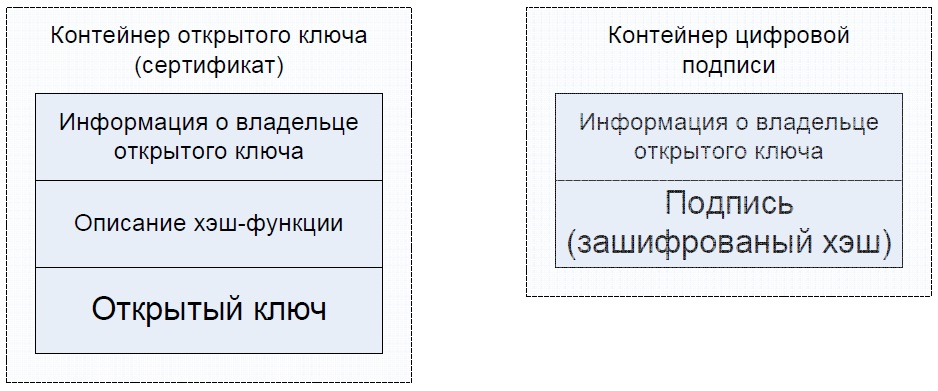
\includegraphics[width=0.7\linewidth]{CryptoPackage}
\caption{Схема контейнера ЭЦП, передаваемого вместе с сообщением.}
\label{fig:CryptoPackage}
\end{figure}
\par Таким образом, данная схема ЭЦП, включает следующие действия. Сторона А для документа вычисляет хеш-функцию, затем полученное значение шифруется с помощью закрытого ключа (private key) получая ЭЦП. Сторона Б получает документ, ЭЦП и сертификат (ссылку на сертификат) стороны А, верифицирует сертификат открытого ключа стороны А в удостоверяющем центре, дешифрует полученную ЭЦП при помощи общего ключа (public key), вычисляет хеш-функцию документа и проверяет с расшифрованым значением. Если сертификат стороны А действителен и проверка прошла успешно, принимается, что документ был подписан стороной А. Данная схема формирования и проверки подписи представлена на \ref{fig:CryptoSchema}.
\begin{figure}[ht]
\centering
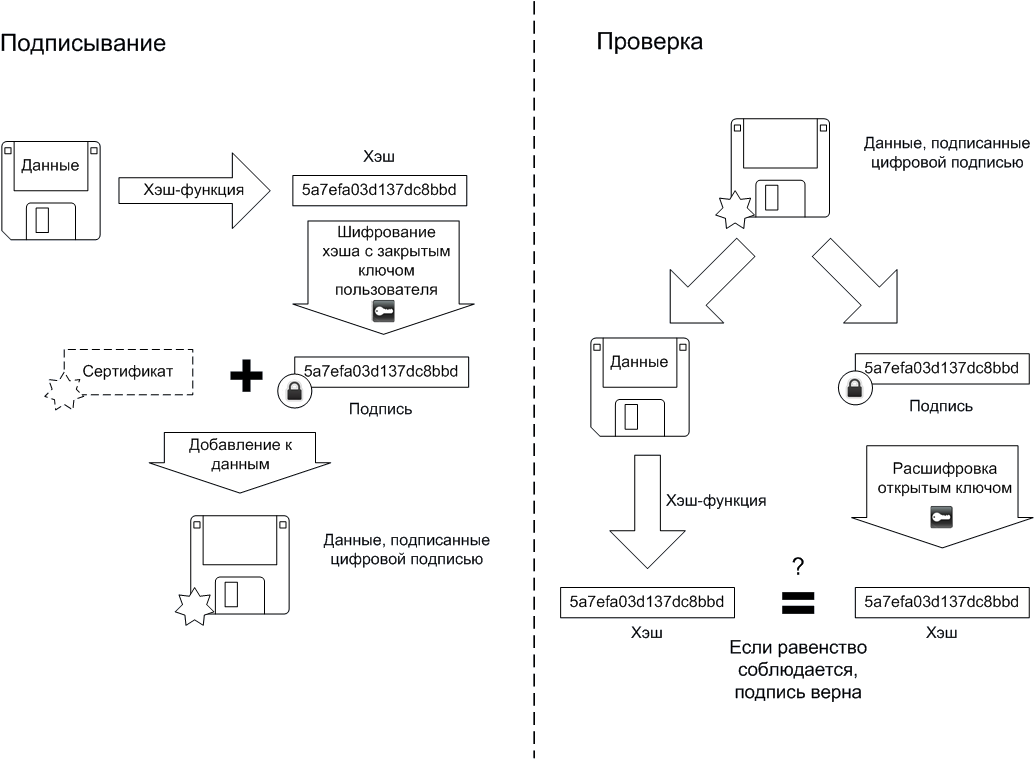
\includegraphics[width=0.9\linewidth]{CryptoSchema}
\caption[Цикл криптографичкеской цифровой подписи]{Схема, иллюстрирующая метод подписи и проверки ЭЦП Криптографические ЦП (КЦП) можно классифицировать по методам шифрования использующимся при их формировании на симметричные и ассиметричные.}
\label{fig:CryptoSchema}
\end{figure}
\subsubsection{ЦП на основе симметричных алгоритмах шифрования}
\par Симметричные схемы ЦП менее распространены чем асимметричные, так как после появления концепции цифровой подписи не удалось реализовать эффективные алгоритмы подписи, основанные на известных в то время симметричных шифрах. Первыми, кто обратил внимание на возможность симметричной схемы цифровой подписи, были основоположники самого понятия ЭП Диффи и Хеллман, которые опубликовали описание алгоритма подписи одного бита с помощью блочного шифра \cite{diffie1976}. Асимметричные схемы цифровой подписи опираются на вычислительно сложные задачи, например на разложение больших чисел на взаимно простые множители. Симметричные схемы основаны на хорошо изученных блочных шифрах. В связи с этим симметричные схемы имеют следующие преимущества:
\begin{itemize}
\item вычислительно менее затратны, по сравнению с аналогичными асимметричными шифрами;
\item возможно простого варьирования криптостойкости шифра;
\end{itemize}
\par Однако у симметричных ЭП есть и ряд недостатков:
\begin{itemize}
\item размер подписи сопоставим с размером подписываемого документа;
\item необходимость использования одноразовых ключей;
\end{itemize}
\subsubsection{ЦП на основе асимметричных алгоритмов шифрования}
\par Асимметричные схемы ЭП относятся к криптосистемам с открытым ключом. в данных схемах цифровой подписи подписание производится с применением закрытого ключа, а проверка подписи — с применением открытого. Схема асимметричного шифрования документа, представлена на \ref{fig:CryptoSchema}. Именно асимметричные схемы получили наибольшее распространение. Протоколы формирования ЦП сертифицированы, стандартизованы и имеют сформированную законодательную базу их применения \cite{gost34.10}. 
\par Общая схема цифровой подписи представленная в \cite{gost34.10} три процесса.
\begin{enumerate}
\item Генерация ключевой пары -- при помощи алгоритма генерации ключа, случайным образом выбирается закрытый ключ и вычисляется соответствующий ему открытый ключ.
\item Формирование подписи -- для заданного электронного документа с помощью закрытого ключа вычисляется подпись.
\item Проверка (верификация) подписи.
\end{enumerate}
\par Для того, чтобы использование цифровой подписи имело смысл, необходимо выполнение двух условий:
верификация подписи должна производиться открытым ключом, соответствующим именно тому закрытому ключу, который использовался при подписании; без обладания закрытым ключом должно быть вычислительно сложно создать легитимную цифровую подпись.














